\documentclass[10pt]{beamer}

\usetheme{Boadilla}
\usecolortheme{default}

\usepackage[T1]{fontenc}
\usepackage{lmodern}
\usepackage{graphicx}
\usepackage{booktabs}
\usepackage{tabularx}
\usepackage{array}
\usepackage{tikz}
\usetikzlibrary{arrows.meta, positioning, fit, shapes.geometric, calc}

\definecolor{RHBlue}{RGB}{21, 57, 97}
\definecolor{RHAccent}{RGB}{0, 123, 138}
\definecolor{RHSoft}{RGB}{235, 243, 247}
\definecolor{RHGray}{RGB}{78, 88, 101}
\definecolor{RHLightGray}{RGB}{245, 247, 250}

\setbeamertemplate{navigation symbols}{}
\setbeamertemplate{itemize item}{\color{RHAccent}\large\textbullet}
\setbeamertemplate{itemize subitem}{\color{RHAccent}\small\textbullet}

\setbeamercolor{title}{fg=RHBlue}
\setbeamercolor{frametitle}{fg=RHBlue, bg=RHSoft}
\setbeamercolor{structure}{fg=RHBlue}
\setbeamercolor{normal text}{fg=black, bg=white}
\setbeamercolor{block title}{fg=white, bg=RHBlue}
\setbeamercolor{block body}{fg=black, bg=RHSoft}
\setbeamercolor{alerted text}{fg=RHAccent}
\setbeamercolor{footline}{fg=white, bg=RHBlue}

\setbeamertemplate{footline}{
  \leavevmode%
  \hbox{%
    \begin{beamercolorbox}[wd=.78\paperwidth,ht=2.7ex,dp=1.2ex,leftskip=1.2em]{footline}%
      \usebeamerfont{author in head/foot}\insertshorttitle
    \end{beamercolorbox}%
    \begin{beamercolorbox}[wd=.22\paperwidth,ht=2.7ex,dp=1.2ex,rightskip=1.2em plus1fil]{footline}%
      \usebeamerfont{date in head/foot}\insertframenumber{} / \inserttotalframenumber
    \end{beamercolorbox}%
  }%
}

\newcommand{\pill}[1]{%
  \tikz[baseline=(X.base)]\node[draw=RHAccent, rounded corners=3pt, fill=RHSoft, inner sep=3pt] (X) {\scriptsize #1};%
}

\newcommand{\goodbox}[2]{
  \begin{block}{#1}
  #2
  \end{block}
}

\newcommand{\func}[1]{\texttt{#1}}

\title[Rolling Horizon Comparison Framework]{Rolling Horizon Comparison Framework}
\subtitle{Product Story, Runtime Architecture, and Agentic Execution}
\author{Sai Madhukiran Kompalli}
\date{March 12, 2026}

\begin{document}

\begin{frame}
  \titlepage
\end{frame}

\section{Why}

\begin{frame}{Why This Framework Exists}
  \begin{itemize}
    \item In rolling-horizon planning, we solve the same business model again and again as time moves forward and new information arrives.
    \item The solver gives a new plan, but business users still ask a second layer of questions:
    \begin{itemize}
      \item What changed in the setup?
      \item How did the plan change?
      \item Can the earlier plan still be used?
      \item What seems to be driving the difference?
    \end{itemize}
    \item Those questions are difficult to answer consistently by hand, especially across large enterprise models.
    \item The RH framework turns that comparison exercise into a reusable product workflow rather than a one-off analyst task.
  \end{itemize}
\end{frame}

\section{Architecture}

%% ============================================================
%%  END-TO-END USER FLOW  –  rescaled to fit slide width
%% ============================================================
\begin{frame}{End-To-End User Flow}
\centering
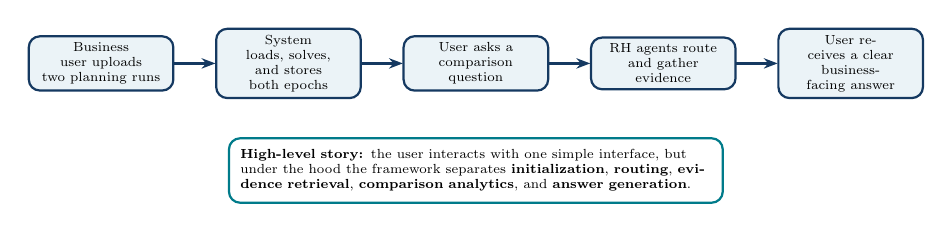
\begin{tikzpicture}[
  scale=0.68,
  transform shape,
  every node/.style={font=\scriptsize},
  flow/.style={draw=RHBlue, rounded corners, thick, fill=RHSoft,
               align=center, minimum width=2.7cm, minimum height=0.95cm,
               text width=2.45cm},
  arr/.style={-{Stealth[length=5pt]}, thick, draw=RHBlue}
]
  \node[flow] (u1)    at (0,    0) {Business user uploads\\two planning runs};
  \node[flow] (init)  at (3.5,  0) {System loads, solves,\\and stores both epochs};
  \node[flow] (u2)    at (7.0,  0) {User asks a\\comparison question};
  \node[flow] (route) at (10.5, 0) {RH agents route\\and gather evidence};
  \node[flow] (u3)    at (14.0, 0) {User receives a clear\\business-facing answer};

  \draw[arr] (u1)   -- (init);
  \draw[arr] (init)  -- (u2);
  \draw[arr] (u2)    -- (route);
  \draw[arr] (route) -- (u3);

  \node[draw=RHAccent, rounded corners, thick, fill=white,
        align=left, text width=8.8cm, inner sep=6pt]
    at (7.0, -2.0) {%
      \textbf{High-level story:} the user interacts with one simple
      interface, but under the hood the framework separates
      \textbf{initialization}, \textbf{routing},
      \textbf{evidence retrieval}, \textbf{comparison analytics},
      and \textbf{answer generation}.};
\end{tikzpicture}
\end{frame}

%% ============================================================
%%  COMPONENT WALKTHROUGH — User-Facing Path  (static version)
%% ============================================================
\begin{frame}{Component Walkthrough: User-Facing Path}
\centering
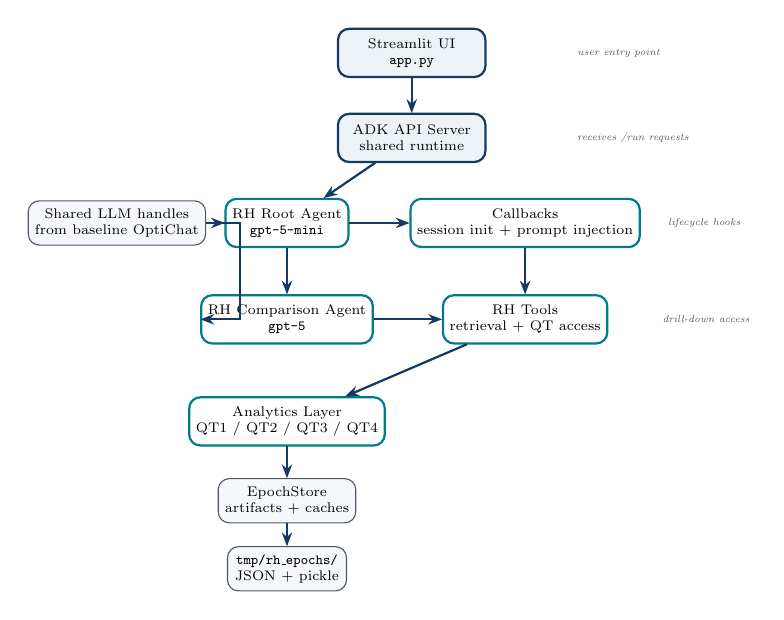
\begin{tikzpicture}[
  scale=0.72,
  transform shape,
  every node/.style={font=\scriptsize},
  box/.style={draw=RHBlue, rounded corners, thick, fill=RHSoft,
              align=center, minimum height=0.85cm, minimum width=2.1cm},
  accentbox/.style={draw=RHAccent, rounded corners, thick, fill=white,
                    align=center, minimum height=0.85cm, minimum width=2.1cm},
  data/.style={draw=RHGray, rounded corners, fill=RHLightGray,
               align=center, minimum height=0.78cm, minimum width=2.1cm},
  arr/.style={-{Stealth[length=5pt]}, thick, draw=RHBlue}
]
  %% Nodes
  \node[box, minimum width=2.6cm]       (ui)        at (6.2, 4.9) {Streamlit UI\\\func{app.py}};
  \node[box, minimum width=2.6cm]       (server)    at (6.2, 3.4) {ADK API Server\\shared runtime};
  \node[data]                           (llm)       at (1.0, 1.9) {Shared LLM handles\\from baseline OptiChat};
  \node[accentbox]                      (root)      at (4.0, 1.9) {RH Root Agent\\\func{gpt-5-mini}};
  \node[accentbox]                      (cmp)       at (4.0, 0.2) {RH Comparison Agent\\\func{gpt-5}};
  \node[accentbox, minimum width=2.6cm] (callbacks) at (8.2, 1.9) {Callbacks\\session init + prompt injection};
  \node[accentbox, minimum width=2.5cm] (tools)     at (8.2, 0.2) {RH Tools\\retrieval + QT access};
  \node[accentbox, minimum width=2.5cm] (analytics) at (4.0,-1.6) {Analytics Layer\\QT1 / QT2 / QT3 / QT4};
  \node[data]                           (store)     at (4.0,-3.0) {EpochStore\\artifacts + caches};
  \node[data]                           (disk)      at (4.0,-4.2) {\func{tmp/rh\_epochs/}\\JSON + pickle};

  %% Arrows
  \draw[arr] (ui)        -- (server);
  \draw[arr] (server)    -- (root);
  \draw[arr] (root)      -- (cmp);
  \draw[arr] (root)      -- (callbacks);
  \draw[arr] (cmp)       -- (tools);
  \draw[arr] (callbacks) -- (tools);
  \draw[arr] (tools)     -- (analytics);
  \draw[arr] (analytics) -- (store);
  \draw[arr] (store)     -- (disk);
  \draw[arr] (llm)       -- (root);
  \draw[arr] (llm.east)  -- ++(0.6,0) |- (cmp.west);

  %% Annotation labels (static, no overlays)
  \node[anchor=west, text=RHGray, font=\tiny\itshape] at (9.0, 4.9)
    {user entry point};
  \node[anchor=west, text=RHGray, font=\tiny\itshape] at (9.0, 3.4)
    {receives /run requests};
  \node[anchor=west, text=RHGray, font=\tiny\itshape] at (10.6, 1.9)
    {lifecycle hooks};
  \node[anchor=west, text=RHGray, font=\tiny\itshape] at (10.5, 0.2)
    {drill-down access};
\end{tikzpicture}
\end{frame}

%% ============================================================
%%  COMPONENT WALKTHROUGH — Backend And Data Path  (static)
%% ============================================================
\begin{frame}{Component Walkthrough: Backend And Data Path}
\centering
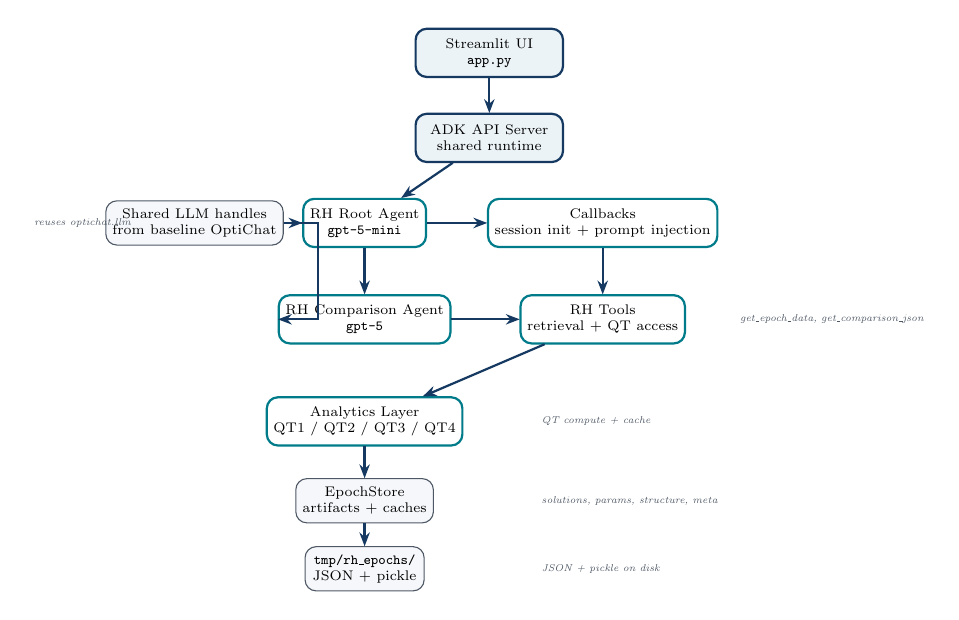
\begin{tikzpicture}[
  scale=0.72,
  transform shape,
  every node/.style={font=\scriptsize},
  box/.style={draw=RHBlue, rounded corners, thick, fill=RHSoft,
              align=center, minimum height=0.85cm, minimum width=2.1cm},
  accentbox/.style={draw=RHAccent, rounded corners, thick, fill=white,
                    align=center, minimum height=0.85cm, minimum width=2.1cm},
  data/.style={draw=RHGray, rounded corners, fill=RHLightGray,
               align=center, minimum height=0.78cm, minimum width=2.1cm},
  arr/.style={-{Stealth[length=5pt]}, thick, draw=RHBlue}
]
  %% Same layout as user-facing path
  \node[box, minimum width=2.6cm]       (ui)        at (6.2, 4.9) {Streamlit UI\\\func{app.py}};
  \node[box, minimum width=2.6cm]       (server)    at (6.2, 3.4) {ADK API Server\\shared runtime};
  \node[data]                           (llm)       at (1.0, 1.9) {Shared LLM handles\\from baseline OptiChat};
  \node[accentbox]                      (root)      at (4.0, 1.9) {RH Root Agent\\\func{gpt-5-mini}};
  \node[accentbox]                      (cmp)       at (4.0, 0.2) {RH Comparison Agent\\\func{gpt-5}};
  \node[accentbox, minimum width=2.6cm] (callbacks) at (8.2, 1.9) {Callbacks\\session init + prompt injection};
  \node[accentbox, minimum width=2.5cm] (tools)     at (8.2, 0.2) {RH Tools\\retrieval + QT access};
  \node[accentbox, minimum width=2.5cm] (analytics) at (4.0,-1.6) {Analytics Layer\\QT1 / QT2 / QT3 / QT4};
  \node[data]                           (store)     at (4.0,-3.0) {EpochStore\\artifacts + caches};
  \node[data]                           (disk)      at (4.0,-4.2) {\func{tmp/rh\_epochs/}\\JSON + pickle};

  %% Arrows
  \draw[arr] (ui)        -- (server);
  \draw[arr] (server)    -- (root);
  \draw[arr] (root)      -- (cmp);
  \draw[arr] (root)      -- (callbacks);
  \draw[arr] (cmp)       -- (tools);
  \draw[arr] (callbacks) -- (tools);
  \draw[arr] (tools)     -- (analytics);
  \draw[arr] (analytics) -- (store);
  \draw[arr] (store)     -- (disk);
  \draw[arr] (llm)       -- (root);
  \draw[arr] (llm.east)  -- ++(0.6,0) |- (cmp.west);

  %% Annotation labels (backend focus)
  \node[anchor=west, text=RHGray, font=\tiny\itshape] at (10.5, 0.2)
    {get\_epoch\_data, get\_comparison\_json};
  \node[anchor=west, text=RHGray, font=\tiny\itshape] at (7.0,-1.6)
    {QT compute + cache};
  \node[anchor=west, text=RHGray, font=\tiny\itshape] at (7.0,-3.0)
    {solutions, params, structure, meta};
  \node[anchor=west, text=RHGray, font=\tiny\itshape] at (7.0,-4.2)
    {JSON + pickle on disk};
  \node[anchor=east, text=RHGray, font=\tiny\itshape] at (0.0, 1.9)
    {reuses optichat.llm};
\end{tikzpicture}
\end{frame}

\begin{frame}{Where RH Sits Inside OptiChat}
  \begin{columns}[T]
    \column{0.48\textwidth}
    \goodbox{Baseline OptiChat}{
      \begin{itemize}
        \item Conversational analysis for one model run
        \item Existing ADK namespace: \func{optichat}
        \item Existing multi-agent workflow
      \end{itemize}
    }
    \column{0.48\textwidth}
    \goodbox{Rolling Horizon Comparison}{
      \begin{itemize}
        \item Comparison between two solved runs
        \item Separate ADK namespace: \func{optichat\_rh}
        \item New analytics, prompts, tools, and persistence layer
      \end{itemize}
    }
  \end{columns}
  \vspace{0.5em}
  \begin{itemize}
    \item Shared pieces: Streamlit UI in \func{app.py}, one ADK API server, and the same LLM handles from \func{optichat.llm}.
    \item Important boundary: RH is a separate comparison stack; it does not reuse the original OptiChat illustrator pipeline.
  \end{itemize}
\end{frame}

\begin{frame}{Repository-Level Implementation Map}
  \scriptsize
  \begin{columns}[T,onlytextwidth]
    \column{0.49\textwidth}
    \goodbox{App \& Agents}{
      \begin{itemize}
        \item \func{optichat\_rh/agent.py}: RH app registration
        \item \func{rh\_comparison/rh\_agent.py}: RH root re-export
        \item \func{agents/rh\_root\_agent.py}: root routing agent
        \item \func{agents/rh\_comparison\_agent.py}: expert answer agent
      \end{itemize}
    }

    \column{0.49\textwidth}
    \goodbox{Prompts \& Orchestration}{
      \begin{itemize}
        \item \func{agents/rh\_prompts.py}: prompt builders and formatters
        \item \func{tools/rh\_callback\_tool.py}: init and prompt injection
        \item \func{tools/epoch\_tools.py}: query routing and drill-down tools
      \end{itemize}
    }
  \end{columns}

  \vspace{0.45em}
  \begin{columns}[T,onlytextwidth]
    \column{0.49\textwidth}
    \goodbox{Data \& Analytics}{
      \begin{itemize}
        \item \func{data\_store/epoch\_store.py}: artifact persistence and caching
        \item \func{analytics/structural\_diff.py}: QT1
        \item \func{analytics/solution\_diff.py}: QT2
        \item \func{analytics/backward\_compat.py}: QT3
        \item \func{analytics/attribution\_analysis.py}: QT4
      \end{itemize}
    }

    \column{0.49\textwidth}
    \goodbox{UI \& Runtime}{
      \begin{itemize}
        \item \func{app.py}: upload flow and RH chat integration
        \item \func{run.sh}: launches Streamlit and the ADK server
        \item Shared LLM handles imported from \func{optichat.llm}
      \end{itemize}
    }
  \end{columns}
\end{frame}

\begin{frame}{Deployment Picture}
  \begin{columns}[T]
    \column{0.48\textwidth}
    \goodbox{Front End}{
      \begin{itemize}
        \item Streamlit app
        \item User uploads two models and optional JSONs
        \item User chats in the RH tab
      \end{itemize}
    }
    \column{0.48\textwidth}
    \goodbox{Back End}{
      \begin{itemize}
        \item One ADK API server
        \item Two app namespaces: baseline and RH
        \item Local solver environment for Pyomo + Gurobi
      \end{itemize}
    }
  \end{columns}
  \vspace{0.5em}
  \begin{itemize}
    \item The important implementation choice is separation: RH is deployed alongside OptiChat, not baked into the baseline path.
  \end{itemize}
\end{frame}

\section{Initialization Flow}

\begin{frame}{Initialization Story: What Happens After Upload}
  \begin{itemize}
    \item The user uploads two model files and optional JSON inputs.
    \item Streamlit builds one RH configuration payload and sends it as the first session message.
    \item The root agent's \func{before\_agent\_callback} intercepts that first message.
    \item Each epoch is loaded, solved once, and converted into stored artifacts.
    \item QT1 is computed immediately.
    \item A manager-friendly model description is generated and stored.
    \item The user receives an initialization summary before asking any question.
  \end{itemize}
\end{frame}

%% ============================================================
%%  INITIALIZATION FLOWCHART  –  refitted coordinates + renamed style
%% ============================================================
\begin{frame}{Initialization Flowchart With Function Names}
\centering
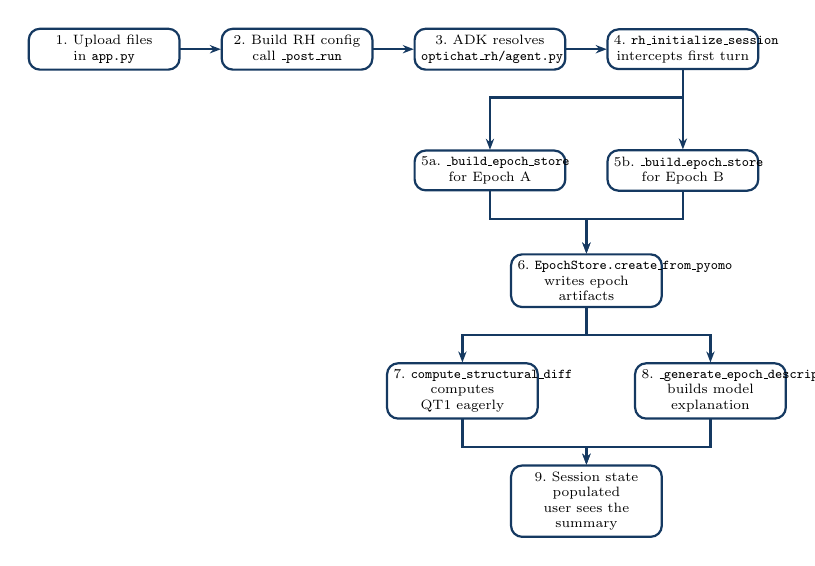
\begin{tikzpicture}[
  scale=0.70,
  transform shape,
  every node/.style={font=\scriptsize},
  stepbox/.style={draw=RHBlue, rounded corners, thick, fill=white,
                  align=center, minimum width=2.6cm, minimum height=0.7cm,
                  text width=2.5cm},
  arr/.style={-{Stealth[length=4pt]}, thick, draw=RHBlue}
]
  %% Row 1  (y = 0)
  \node[stepbox] (upload) at (0,    0)  {1.~Upload files\\in \func{app.py}};
  \node[stepbox] (config) at (3.5,  0)  {2.~Build RH config\\call \func{\_post\_run}};
  \node[stepbox] (root)   at (7.0,  0)  {3.~ADK resolves\\\func{optichat\_rh/agent.py}};
  \node[stepbox] (init)   at (10.5, 0)  {4.~\func{rh\_initialize\_session}\\intercepts first turn};

  %% Row 2  (y = -2.2)
  \node[stepbox] (builda) at (7.0, -2.2)  {5a.~\func{\_build\_epoch\_store}\\for Epoch~A};
  \node[stepbox] (buildb) at (10.5,-2.2)  {5b.~\func{\_build\_epoch\_store}\\for Epoch~B};

  %% Row 3  (y = -4.2)
  \node[stepbox] (persist) at (8.75,-4.2) {6.~\func{EpochStore.create\_from\_pyomo}\\writes epoch artifacts};

  %% Row 4  (y = -6.2)
  \node[stepbox] (qt1)  at (6.5, -6.2)  {7.~\func{compute\_structural\_diff}\\computes QT1 eagerly};
  \node[stepbox] (desc) at (11.0,-6.2)  {8.~\func{\_generate\_epoch\_description}\\builds model explanation};

  %% Row 5  (y = -8.2)
  \node[stepbox] (ready) at (8.75,-8.2) {9.~Session state populated\\user sees the summary};

  %% Arrows – Row 1
  \draw[arr] (upload) -- (config);
  \draw[arr] (config) -- (root);
  \draw[arr] (root)   -- (init);

  %% Row 1 → Row 2
  \draw[arr] (init.south) -- ++(0,-0.5) -| (builda.north);
  \draw[arr] (init.south) -- ++(0,-0.5) -| (buildb.north);

  %% Row 2 → Row 3
  \draw[arr] (builda.south) -- ++(0,-0.5) -| (persist.north);
  \draw[arr] (buildb.south) -- ++(0,-0.5) -| (persist.north);

  %% Row 3 → Row 4
  \draw[arr] (persist.south) -- ++(0,-0.5) -| (qt1.north);
  \draw[arr] (persist.south) -- ++(0,-0.5) -| (desc.north);

  %% Row 4 → Row 5
  \draw[arr] (qt1.south)  -- ++(0,-0.5) -| (ready.north);
  \draw[arr] (desc.south) -- ++(0,-0.5) -| (ready.north);
\end{tikzpicture}
\end{frame}

\begin{frame}{What Gets Stored For Each Epoch}
  \begin{columns}[T]
    \column{0.50\textwidth}
    \goodbox{Core Files}{
      \begin{itemize}
        \item \func{solution.json}
        \item \func{params.json}
        \item \func{structure.json}
        \item \func{meta.json}
        \item \func{model.pkl}
      \end{itemize}
    }
    \column{0.46\textwidth}
    \goodbox{Purpose}{
      \begin{itemize}
        \item Preserve one solved run
        \item Avoid repeated heavy work
        \item Support drill-down questions later
        \item Survive process restarts
      \end{itemize}
    }
  \end{columns}
  \vspace{0.5em}
  \begin{itemize}
    \item Comparison results are stored separately under a pairwise comparison directory as \func{qt1\_structural.json}, \func{qt2\_solution.json}, \func{qt3\_backward.json}, and \func{qt4\_attribution.json}.
  \end{itemize}
\end{frame}

\begin{frame}{What Is Inside Those Artifacts}
  \small
  \begin{tabularx}{\textwidth}{>{\raggedright\arraybackslash}p{0.22\textwidth} X}
    \toprule
    \textbf{Artifact} & \textbf{Contents} \\
    \midrule
    \func{solution.json} & Objective value, variable values, binary/integer flags, constraint binding status, and LP duals when available. \\
    \func{params.json} & Parameter family values for the uploaded run. \\
    \func{structure.json} & Sets, family-level schema, component docs, objective metadata, and model description inputs. \\
    \func{meta.json} & Label, solve status, counts, objective sense, and source file metadata. \\
    \func{description.txt} & The reusable business-facing model explanation shown to the user and injected into later prompts. \\
    \bottomrule
  \end{tabularx}
\end{frame}

\begin{frame}{Why The Artifact Layer Matters}
  \begin{itemize}
    \item The expensive solve happens once during initialization.
    \item Most later questions are answered from stored artifacts, cached comparison results, or lightweight formatting logic.
    \item This makes the framework more stable, faster on repeated questions, and easier to explain from an architecture perspective.
    \item It also gives us a clean separation between:
    \begin{itemize}
      \item solver-backed computation
      \item persisted comparison data
      \item LLM answer generation
    \end{itemize}
  \end{itemize}
\end{frame}

\section{Question-Time Flow}

\begin{frame}{Question-Time Story: The Simple Version}
  \begin{itemize}
    \item A user asks a question after the session is initialized.
    \item The root agent classifies what kind of question it is.
    \item The comparison agent receives the same question, but now with the right context and tools.
    \item The callback may compute a missing comparison result if the question needs one.
    \item The comparison agent answers directly, or uses retrieval tools for extra detail.
  \end{itemize}
\end{frame}

%% ============================================================
%%  QUERY-TIME FLOWCHART  –  refitted + renamed style
%% ============================================================
\begin{frame}{Query-Time Flowchart With Function Names}
\centering
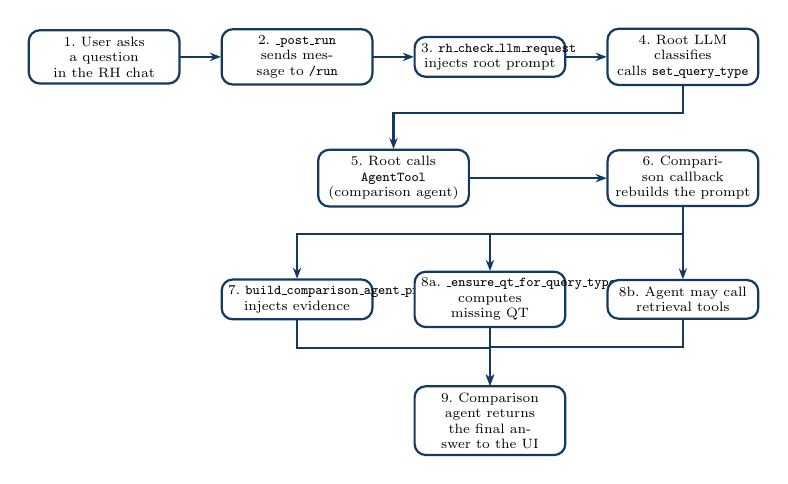
\begin{tikzpicture}[
  scale=0.70,
  transform shape,
  every node/.style={font=\scriptsize},
  stepbox/.style={draw=RHBlue, rounded corners, thick, fill=white,
                  align=center, minimum width=2.6cm, minimum height=0.7cm,
                  text width=2.5cm},
  arr/.style={-{Stealth[length=4pt]}, thick, draw=RHBlue}
]
  %% Row 1  (y = 0)
  \node[stepbox] (ask)      at (0,    0) {1.~User asks a question\\in the RH chat};
  \node[stepbox] (run)      at (3.5,  0) {2.~\func{\_post\_run}\\sends message to \func{/run}};
  \node[stepbox] (rootcb)   at (7.0,  0) {3.~\func{rh\_check\_llm\_request}\\injects root prompt};
  \node[stepbox] (classify) at (10.5, 0) {4.~Root LLM classifies\\calls \func{set\_query\_type}};

  %% Row 2  (y = -2.2)
  \node[stepbox] (delegate)  at (5.25,-2.2) {5.~Root calls \func{AgentTool}\\(comparison agent)};
  \node[stepbox] (cmpcb)     at (10.5, -2.2) {6.~Comparison callback\\rebuilds the prompt};

  %% Row 3  (y = -4.4)
  \node[stepbox] (prompt) at (3.5, -4.4) {7.~\func{build\_comparison\_agent\_prompt}\\injects evidence};
  \node[stepbox] (qt)     at (7.0, -4.4) {8a.~\func{\_ensure\_qt\_for\_query\_type}\\computes missing QT};
  \node[stepbox] (tool)   at (10.5,-4.4) {8b.~Agent may call\\retrieval tools};

  %% Row 4  (y = -6.6)
  \node[stepbox] (answer) at (7.0,-6.6) {9.~Comparison agent returns\\the final answer to the UI};

  %% Arrows – Row 1
  \draw[arr] (ask)    -- (run);
  \draw[arr] (run)    -- (rootcb);
  \draw[arr] (rootcb) -- (classify);

  %% Row 1 → Row 2
  \draw[arr] (classify.south) -- ++(0,-0.5) -| (delegate.north);
  \draw[arr] (delegate) -- (cmpcb);

  %% Row 2 → Row 3
  \draw[arr] (cmpcb.south) -- ++(0,-0.5) -| (prompt.north);
  \draw[arr] (cmpcb.south) -- ++(0,-0.5) -| (qt.north);
  \draw[arr] (cmpcb.south) -- ++(0,-0.5) -| (tool.north);

  %% Row 3 → Row 4
  \draw[arr] (prompt.south) -- ++(0,-0.5) -| (answer.north);
  \draw[arr] (qt.south)     -- (answer.north);
  \draw[arr] (tool.south)   -- ++(0,-0.5) -| (answer.north);
\end{tikzpicture}
\end{frame}

\begin{frame}{Root Agent And Comparison Agent: Role Separation}
  \begin{columns}[T]
    \column{0.48\textwidth}
    \goodbox{Root Agent}{
      \begin{itemize}
        \item Lightweight routing agent
        \item Model: \func{gpt-5-mini}
        \item Tools:
        \begin{itemize}
          \item \func{set\_query\_type(...)}
          \item \func{AgentTool(comparison\_agent)}
        \end{itemize}
        \item Job: choose the question type and delegate
      \end{itemize}
    }
    \column{0.48\textwidth}
    \goodbox{Comparison Agent}{
      \begin{itemize}
        \item Expert answering agent
        \item Model: \func{gpt-5}
        \item Tools:
        \begin{itemize}
          \item \func{get\_epoch\_data(...)}
          \item \func{get\_comparison\_json(...)}
        \end{itemize}
        \item Job: answer with the right evidence and drill-down as needed
      \end{itemize}
    }
  \end{columns}
\end{frame}

\begin{frame}{The Four Decisions Made For Each User Question}
  \begin{columns}[T]
    \column{0.49\textwidth}
    \goodbox{Decision 1: Query Type}{
      \begin{itemize}
        \item GENERAL
        \item RETRIEVAL
        \item MODEL DESCRIPTION
        \item STRUCTURAL CHANGE
        \item SOLUTION DIFF
        \item BACKWARD COMPAT
        \item ATTRIBUTION
      \end{itemize}
    }
    \column{0.49\textwidth}
    \goodbox{Decision 2--4: Answer Shape}{
      \begin{itemize}
        \item Focus: broad vs.\ focused
        \item Subfocus: setup, drivers, reuse check, etc.
        \item Answer profile: detailed vs.\ summary
      \end{itemize}
    }
  \end{columns}
  \vspace{0.5em}
  \begin{itemize}
    \item Query type is chosen by the root LLM.
    \item Focus, subfocus, and answer profile are chosen by Python helper logic in \func{rh\_prompts.py}.
  \end{itemize}
\end{frame}

\begin{frame}{How The Final Comparison Prompt Is Built}
  \small
  \begin{tabularx}{\textwidth}{>{\raggedright\arraybackslash}p{0.25\textwidth} X}
    \toprule
    \textbf{Prompt block} & \textbf{What it contributes} \\
    \midrule
    Base prompt & Current user question, detected focus, answer profile, and general response rules. \\
    Epoch metadata block & Labels, status, objective values, counts, and high-level run facts. \\
    Epoch description block & The reusable model explanation built at initialization time. \\
    Query-specific block & QT1, QT2, QT3, QT4, or no injected analysis for retrieval-only questions. \\
    Guidance block & Style instructions plus broad/focused and detailed/summary answer policy. \\
    Tool block & Reminds the comparison agent that it can retrieve more exact data when needed. \\
    \bottomrule
  \end{tabularx}
\end{frame}

\begin{frame}{What Happens On A Retrieval Question}
  \begin{itemize}
    \item The root agent classifies the question as \pill{RETRIEVAL}.
    \item The comparison callback does \textbf{not} compute QT2, QT3, or QT4 just for that question.
    \item The comparison prompt mostly provides guidance and model context.
    \item The comparison agent then calls retrieval tools if it needs exact values, counts, memberships, or family-level details.
  \end{itemize}
  \vspace{0.5em}
  \goodbox{Important Implementation Detail}{
    Retrieval reads from stored epoch artifacts such as \func{solution.json}, \func{params.json}, and \func{structure.json}. It does not re-solve the model.
  }
\end{frame}

\begin{frame}{Retrieval Function Chain}
  \scriptsize
  \begin{tabularx}{\textwidth}{>{\raggedright\arraybackslash}p{0.32\textwidth} X}
    \toprule
    \textbf{Step} & \textbf{Function path} \\
    \midrule
    Message arrives & \func{app.py:\_post\_run(...)} \\
    Query type stored & \func{epoch\_tools.py:set\_query\_type(...)} \\
    Retrieval prompt built & \func{rh\_callback\_tool.py:\allowbreak{}rh\_check\_llm\_request(...)}\newline then \func{rh\_prompts.py:\allowbreak{}build\_comparison\_agent\_prompt(...)} \\
    Epoch data requested & \func{epoch\_tools.py:\allowbreak{}get\_epoch\_data(...)} \\
    Stored artifact accessed & \func{EpochStore}: \func{get\_solution()}, \func{get\_params()}, \func{get\_structure()}, \func{get\_variable\_family()}, \func{get\_param\_family()} \\
    Answer returned & Comparison agent writes the response; UI strips tool chatter and shows the final text \\
    \bottomrule
  \end{tabularx}
  \vspace{0.5em}
  \begin{itemize}
    \item Exact family lookup is tool-level exact match.
    \item The LLM maps user wording to the actual family name using docs and labels.
  \end{itemize}
\end{frame}

\begin{frame}{When Do We Solve Again?}
  \begin{columns}[T]
    \column{0.48\textwidth}
    \goodbox{No New Solve Needed}{
      \begin{itemize}
        \item Initialization summary
        \item Model description questions
        \item Structural change questions
        \item Retrieval questions
        \item Most solution-difference questions
      \end{itemize}
    }
    \column{0.48\textwidth}
    \goodbox{May Trigger Solver Work}{
      \begin{itemize}
        \item QT3 backward compatibility
        \item QT4 attribution when extra LP information is needed
      \end{itemize}
    }
  \end{columns}
  \vspace{0.5em}
  \begin{itemize}
    \item So the framework is mostly artifact-driven after initialization; only the deeper analyses may trigger fresh solver-backed work.
  \end{itemize}
\end{frame}

\begin{frame}{Caching Strategy}
  \begin{itemize}
    \item Epoch artifacts are cached in two ways:
    \begin{itemize}
      \item in process memory during the active server session
      \item on disk under \func{tmp/rh\_epochs/}
    \end{itemize}
    \item QT results are cached in session state and also stored on disk for repeated use.
    \item This means:
    \begin{itemize}
      \item repeated questions are faster
      \item server restarts can recover from disk
      \item the answer prompt can be rebuilt every time without recomputing everything
    \end{itemize}
  \end{itemize}
\end{frame}

\section{Analytical Services}

\begin{frame}{The Framework Answers Five Types Of Need}
  \scriptsize
  \begin{tabularx}{\textwidth}{>{\raggedright\arraybackslash}p{0.12\textwidth} >{\raggedright\arraybackslash}p{0.23\textwidth} X >{\raggedright\arraybackslash}p{0.18\textwidth}}
    \toprule
    \textbf{Mode} & \textbf{User need} & \textbf{What the framework provides} & \textbf{When computed} \\
    \midrule
    QT1 & What changed in the setup? & Scope changes, input-data changes, option changes, rule-family changes & Eagerly at initialization \\
    QT2 & How did the plan change? & Plan differences, activity shifts, additions, removals, binding changes & On demand and cached \\
    QT3 & Can the old plan still work? & Feasible or infeasible reuse check and minimum rule changes needed & On demand and cached \\
    QT4 & What seems to have driven the change? & Explanation of changed priorities, limits, availability, and effectiveness & On demand and cached \\
    Retrieval & What is the value of a specific thing? & Exact counts, memberships, values, summaries, and family drill-down & Tool-driven at question time \\
    \bottomrule
  \end{tabularx}
\end{frame}

\begin{frame}{QT1: Structural And Input-Data Change Analysis}
  \begin{itemize}
    \item QT1 compares the extracted model artifacts from both runs.
    \item It separates two different ideas that users often mix together:
    \begin{itemize}
      \item formulation change: new or removed set families, decision families, or rule families
      \item run-data change: new members, changed parameter values, changed planning coverage
    \end{itemize}
    \item This matters because many business users ask ``what changed structurally?'' when the true answer is ``the model stayed the same, but the data changed.''
    \item QT1 is solver-free after initialization because it works on stored artifacts.
  \end{itemize}
\end{frame}

\begin{frame}{QT2: Solution Difference Analysis}
  \begin{itemize}
    \item QT2 compares the two solved plans, not just the objective values.
    \item It looks at:
    \begin{itemize}
      \item changes in activity by decision family
      \item movements across overlapping dimensions
      \item additions and removals caused by new periods or new options
      \item binding-status changes on constraints
    \end{itemize}
    \item The answer layer is designed to say first what the plan is doing differently, then add supporting numbers and drivers if the question asks for them.
    \item Detailed variable-family comparisons can be requested without flooding the base prompt.
  \end{itemize}
\end{frame}

\begin{frame}{QT3: Backward Compatibility}
  \begin{itemize}
    \item QT3 answers the practical question: can the earlier plan still be used under today's rules?
    \item Implementation logic:
    \begin{itemize}
      \item fix all overlapping decisions from the earlier run onto the later model
      \item leave later-only decisions free
      \item solve the later model under those locks
    \end{itemize}
    \item If feasible, report the forced outcome and the gap versus the later optimum.
    \item If infeasible, diagnose which current rules block reuse and how much those rules would need to change.
  \end{itemize}
\end{frame}

\begin{frame}{QT4: Attribution Analysis}
  \begin{itemize}
    \item QT4 is not claiming perfect causality.
    \item It provides a structured explanation of what appears to have driven the plan change.
    \item The analysis connects:
    \begin{itemize}
      \item changed parameters
      \item changed bottlenecks or shadow-price landscape
      \item changed decision patterns
    \end{itemize}
    \item The answer that reaches the user is grouped into business buckets such as changed priorities, changed limits, changed availability, and changed effectiveness.
  \end{itemize}
\end{frame}

\section{Explanation Layer}

\begin{frame}{How We Generate The Initial Model Description}
  \begin{itemize}
    \item The initial description is now deterministic and template-driven.
    \item We do \textbf{not} simply dump raw Pyomo \func{doc=} strings.
    \item Instead, we use those docs as semantic inputs and write a structured explanation with:
    \begin{itemize}
      \item an overview paragraph
      \item sets
      \item parameters
      \item variables
      \item constraints
      \item objective
    \end{itemize}
    \item This gives a more textbook-style explanation for non-expert users.
  \end{itemize}
\end{frame}

\begin{frame}{How Docs Become Business Language}
  \begin{columns}[T]
    \column{0.48\textwidth}
    \goodbox{What We Read}{
      \begin{itemize}
        \item \func{ConcreteModel.doc}
        \item \func{Set.doc}
        \item \func{Param.doc}
        \item \func{Var.doc}
        \item \func{Constraint.doc}
        \item \func{Objective.doc}
      \end{itemize}
    }
    \column{0.48\textwidth}
    \goodbox{What We Build}{
      \begin{itemize}
        \item A clear intro paragraph
        \item Full sentence entries per component
        \item Natural phrasing from index metadata
        \item A reusable description block for later prompts
      \end{itemize}
    }
  \end{columns}
  \vspace{0.5em}
  \begin{itemize}
    \item Better model docs improve everything: initialization quality, retrieval accuracy, and business-facing later answers.
  \end{itemize}
\end{frame}

\begin{frame}{How We Keep Answers Adapted To The User's Question}
  \begin{itemize}
    \item Broad questions get a more report-like answer.
    \item Focused questions stay narrow, but still include enough context to be understandable.
    \item Small relevant context gets a \func{detailed} profile.
    \item Large relevant context gets a \func{summary} profile with full family-level coverage and selective examples.
    \item Retrieval answers are direct first, then lightly contextual unless the user explicitly wants just the value.
  \end{itemize}
\end{frame}

\begin{frame}{Why We Needed Size-Aware Prompting}
  \begin{itemize}
    \item For small models, the system can answer directly and in depth.
    \item For large enterprise models, dumping every changed item into the prompt or answer is counterproductive.
    \item The framework therefore chooses between:
    \begin{itemize}
      \item \func{detailed}: fuller coverage, more examples
      \item \func{summary}: complete family-level overview, selective examples, drill-down available
    \end{itemize}
    \item This is how we keep answers informative without overwhelming the user or the model context window.
  \end{itemize}
\end{frame}

\begin{frame}{What Makes This Agentic Rather Than A Single Prompt}
  \begin{columns}[T]
    \column{0.48\textwidth}
    \goodbox{Agentic Behaviors}{
      \begin{itemize}
        \item Separate routing and answering roles
        \item Dynamic prompt rebuilding
        \item Tool use only when needed
        \item On-demand analytical computation
      \end{itemize}
    }
    \column{0.48\textwidth}
    \goodbox{Why That Matters}{
      \begin{itemize}
        \item Different question types need different evidence
        \item Large models need scoped retrieval
        \item Repeated questions benefit from caches
        \item We can keep the same user interface while changing the internal path
      \end{itemize}
    }
  \end{columns}
\end{frame}

\section{Operational Considerations}

\begin{frame}{How The Framework Scales To Larger Models}
  \begin{itemize}
    \item Tool responses are capped so a single tool call does not blow up the prompt.
    \item The system works at family level first and drills into individual items only when needed.
    \item Prompt injection is selective:
    \begin{itemize}
      \item always include the reusable model explanation
      \item inject only the relevant QT summary
      \item call tools if the user needs more exact detail
    \end{itemize}
    \item This lets the same framework support both toy examples and larger enterprise problems.
  \end{itemize}
\end{frame}

\begin{frame}{Quality And Reliability Guardrails}
  \begin{itemize}
    \item Initialization returns a deterministic summary even before the LLM starts answering.
    \item Prompt formatters convert raw analytics into cleaner evidence blocks before the comparison agent sees them.
    \item Session state stores the current query type and cached results, so the answer path is reproducible within a session.
    \item On-disk storage makes the system more resilient to server restarts.
    \item The answer layer is explicitly tuned to avoid raw optimization jargon in user-facing responses.
  \end{itemize}
\end{frame}

\begin{frame}{Current Design Boundaries}
  \begin{itemize}
    \item RH is a separate comparison framework, not a modification of baseline OptiChat's illustrator flow.
    \item Exact retrieval of a family still depends on the LLM mapping business wording to the true family name.
    \item Good Pyomo \func{doc=} strings materially improve the quality of both the model explanation and the later answers.
    \item QT3 and parts of QT4 still depend on the local solver environment being available.
    \item The framework is strong on explanation and comparison, but it is only as good as the uploaded models, data, and metadata.
  \end{itemize}
\end{frame}

\section{Recap}

\begin{frame}{End-To-End Summary}
  \begin{enumerate}
    \item The user uploads two models and optional JSON inputs.
    \item The RH initialization callback loads both epochs, solves them once, and persists artifacts.
    \item QT1 is computed eagerly and the model description is generated immediately.
    \item Later questions are routed by a root agent and answered by a comparison agent.
    \item The comparison prompt is rebuilt for every question from the right metadata, summaries, and tools.
    \item Most answers come from stored artifacts and cached comparison results rather than re-solving the model.
    \item The final output is rewritten for a non-expert audience in business language.
  \end{enumerate}
\end{frame}

\begin{frame}{Takeaway}
  \begin{columns}[T]
    \column{0.48\textwidth}
    \goodbox{What We Built}{
      \begin{itemize}
        \item A comparison layer on top of OptiChat
        \item Artifact-driven analytics for two model runs
        \item Agentic routing, retrieval, and explanation generation
      \end{itemize}
    }
    \column{0.48\textwidth}
    \goodbox{Why It Matters}{
      \begin{itemize}
        \item Faster comparison workflow
        \item Better non-technical communication
        \item Reusable framework for multiple model classes
      \end{itemize}
    }
  \end{columns}
  \vspace{0.7em}
  \centering
  \pill{separate RH app}
  \hspace{0.4em}
  \pill{artifact-driven}
  \hspace{0.4em}
  \pill{query-aware prompts}
  \hspace{0.4em}
  \pill{business-facing answers}
\end{frame}

\section{Illustrative Example}

\begin{frame}{Illustrative Example Placeholder: Setup}
  \begin{block}{Use This Slide For}
    \begin{itemize}
      \item the business problem being compared
      \item what Epoch A represents
      \item what Epoch B represents
      \item the user's first question
    \end{itemize}
  \end{block}
  \vfill
  \centering
  \Large Insert example setup here
  \vfill
\end{frame}

\begin{frame}{Illustrative Example Placeholder: RH Output}
  \begin{block}{Use This Slide For}
    \begin{itemize}
      \item one initialization summary excerpt
      \item one broad comparison answer
      \item one focused follow-up answer
    \end{itemize}
  \end{block}
  \vfill
  \centering
  \Large Insert example outputs here
  \vfill
\end{frame}

\begin{frame}{Illustrative Example Placeholder: Business Takeaway}
  \begin{block}{Use This Slide For}
    \begin{itemize}
      \item what changed in business terms
      \item how the framework helped explain it
      \item transition into a live demo or discussion
    \end{itemize}
  \end{block}
  \vfill
  \centering
  \Large Insert example takeaway here
  \vfill
\end{frame}

\begin{frame}{Discussion}
  \centering
  \Large Questions
  \vspace{1em}

  \normalsize
  Suggested discussion prompts:
  \begin{itemize}
    \item Which business models are the best first candidates for RH comparison?
    \item Where should this sit in the planning workflow?
    \item What governance do we want for business-facing explanation quality?
    \item Which parts should become productized first: upload flow, answers, or analytics?
  \end{itemize}
\end{frame}

\end{document}